% !TEX TS-program = pdflatex
% !TEX encoding = UTF-8 Unicode

% This is a simple template for a LaTeX document using the "article" class.
% See "book", "report", "letter" for other types of document.

\documentclass[10pt]{article} % use larger type; default would be 10pt


%begin personal config
\usepackage{extarrows}
\usepackage{chemarrow}
\usepackage{amsthm}
\usepackage{amsmath}
\usepackage{amssymb}
\usepackage{calc} 
\usepackage{forloop}
\usepackage{framed}
\usepackage{graphicx}
\usepackage{wrapfig}
\usepackage{xcolor}
\usepackage{mathpazo}
\usepackage{lastpage}
\usepackage{totcount}
\usepackage[hmargin=2.5cm,vmargin=2.5cm]{geometry}

\newtotcounter{calctotalmarks}
\setcounter{calctotalmarks}{0} 
\newcounter{forloopcounter}
\newcommand{\putansline}[2]{\setcounter{forloopcounter}{1}\forloop{forloopcounter}{0}{\value{forloopcounter}< #1}{\par\vspace{\the\baselineskip}\dotfill}[#2]\addtocounter{calctotalmarks}{#2}}

\theoremstyle{definition}
\newtheorem{conclusion}{Conclusion}[subsection]
\theoremstyle{definition}
\newtheorem{definition}{Definition}[subsection]
%finish personal config


\usepackage[utf8]{inputenc} % set input encoding (not needed with XeLaTeX)

%%% Examples of Article customizations
% These packages are optional, depending whether you want the features they provide.
% See the LaTeX Companion or other references for full information.

%%% PAGE DIMENSIONS
\usepackage{geometry} % to change the page dimensions
\geometry{a4paper} % or letterpaper (US) or a5paper or....
% \geometry{margin=2in} % for example, change the margins to 2 inches all round
% \geometry{landscape} % set up the page for landscape
%   read geometry.pdf for detailed page layout information

\usepackage{graphicx} % support the \includegraphics command and options

% \usepackage[parfill]{parskip} % Activate to begin paragraphs with an empty line rather than an indent

%%% PACKAGES
\usepackage{booktabs} % for much better looking tables
\usepackage{array} % for better arrays (eg matrices) in maths
\usepackage{paralist} % very flexible & customisable lists (eg. enumerate/itemize, etc.)
\usepackage{verbatim} % adds environment for commenting out blocks of text & for better verbatim
\usepackage{subfig} % make it possible to include more than one captioned figure/table in a single float
% These packages are all incorporated in the memoir class to one degree or another...

%%% HEADERS & FOOTERS
\usepackage{fancyhdr} % This should be set AFTER setting up the page geometry
\pagestyle{plain} % options: empty , plain , fancy
\renewcommand{\headrulewidth}{0pt} % customise the layout...
\lhead{}\chead{}\rhead{}
\lfoot{}\cfoot{\thepage}\rfoot{}

%%% SECTION TITLE APPEARANCE
\usepackage{sectsty}
\allsectionsfont{\sffamily\mdseries\upshape} % (See the fntguide.pdf for font help)
% (This matches ConTeXt defaults)

%%% ToC (table of contents) APPEARANCE
\usepackage[nottoc,notlof,notlot]{tocbibind} % Put the bibliography in the ToC
\usepackage[titles,subfigure]{tocloft} % Alter the style of the Table of Contents
\renewcommand{\cftsecfont}{\rmfamily\mdseries\upshape}
\renewcommand{\cftsecpagefont}{\rmfamily\mdseries\upshape} % No bold!

%%% END Article customizations

%%% The "real" document content comes below...

\title{Distant Supervision for Relation Extraction}
\author{Zhen Wang (v-zw)}
%\date{} % Activate to display a given date or no date (if empty),
         % otherwise the current date is printed 

\begin{document}
\maketitle
\section{Background}
As the amount of electronic text corpora becomes larger and larger, discovering structured information from unstructured natural language attracts more and more attention from both academic and industry communities. 
Currently, the structured information in which we are interested is ordered binary \emph{relation} such as 'CEO-of', 'Born-in', 'Contains', etc. 
We call a concrete ordered entity pair \emph{relation instance}. 
For instance, '(Steve Jobs, Apple)' is an instance of the relation 'CEO-of'. 
Relation extraction is tasked with harvesting many unseen relation instances from a text corpus. 
As a sub-task of information extraction, most previous works assume that there is an oracle which is capable to detect named entities from input text snippets and classify each entity to one of pre-defined classes (i.e., entity types). 
Then they focus on judging whether an entity pair posseses some relation. 
In a supervised learning scenario, a training set is manually annotated where an observation is an entity pair as well as its feature representation and label is the relation connecting the two entities. 
Since building such a training set is costly and not practical for scaling up, supervised learning for relation extraction is limited to small dataset or specific domain. 
On the other hand, unsupervised learning aggregates similar relation instances together by discovering the intrinsic strucrue within their feature space. 
Thus, unsupervised learning for relation extraction can be applied to very large text corpora. 
However, it is difficult to map each cluster of relation instances to a canonical realtion type defined in existed knowledge bases (KB) and thus novel relation instances can not be immediately inserted into KB. 
Distant supervision (DS)~\cite{mintz} provdies a paradigm to heuristically label a large corpus without human labor for training a relation extractor. 
DS assumes that given 
%The larger a text corpus is, the larger the training set generated by DS will be. 
%This promising feature results from the assumption of DS that given 
\begin{itemize}
\item $\Sigma$, a large corpus e.g., Wikipedia articles, NYT, etc. 
\item $E$, a set of entities mentioned in $\Sigma$ e.g., 'Barack Obama', 'Gone with the wind', etc. 
\item $R$, a set of relation types e.g., 'CEO-of', 'Born-in', etc. 
\item $\Delta$, a set of ground relation instances of relations in $R$ e.g., 'CEO-of(Steve Ballman, Microsoft)', 'Born-in(Barack Obama, Ohio)', etc. 
\item $T$, a set of entity types e.g., 'PER', 'ORG, 'LOC', etc, as well as type signature $r(E_1,E_2)$ for relations e.g., '(PER, LOC)' for 'Born-in'. 
\end{itemize}
for any sentence $s\in\Sigma$ that contains a pair of entity $(e_1,e_2)$, if $\exists{}r\in{}R$ such that $r(e_1,e_2)\in\Delta$, regard $s$ as an expression of relation $r$. 
Specifically, for each sentence $s\in\Sigma$, they use Stanford's named entity tagger to detect all named entities in $s$. 
For each entity pair, if $\exists{}r\in{}R$ such that $r(e_1,e_2)\in\Delta$, they extract both lexical and syntactic features from $s$ w.r.t. $(e1,e2)$ and combine features extracted from \emph{all} mentions of $(e_1,e_2)$ 
to form a positive example $(x_i,y_i)$ where $x_i$ is the aggregated features of $(e_1,e_2)$ and $y_i=r$. 
If $\forall{}r\in{}R,r(e_1,e_2)\notin\Delta$, a negative example is constructed. 
The larger a text corpus is, the larger the training set generated by DS will be. 
Although this promising property has made DS for relation extraction one of the hottest research topics, it still posseses some challenging problems. 
In this survey, we will analysis these problems and discuss related works that made efforts to solve these problems. 



\section{Challenging Problems}
Firstly, the assumption of the existence of a perfect NER tagger does not make sense. 
Most of previous works made use of the Stanford NER tagger with a 4-classes label set $\{\text{'PER', 'ORG', 'LOC', 'MISC', 'NONE'}\}$. 
I thought up 30 entities (each category has 10 entities) include 'Hong Kong', 'Los Angeles', 'Opec', 'NCAA', 'Nixon' and 'Bill Gates', etc.
Then I checked their NER tags within each mention of them. 
According to my observation, the Stanford NER tagger can classify entities without ambiguity into their appropriate classes with high accuracy (about 92\%). 
However, there are many ambiguous names which refer to different entities under different contexts. 
For example, 'Barcelona' may be a city or a football club where the corresponding NER tag should be 'LOC' or 'ORG'. 
In 72 mentions, the tag of 'Barcelona' is 'ORG' but only 35 of these mentions are indeed talking about that famous football club. 
On the other hand, there are 65 mentions in which 'Barcelona' refers to the city in Spain but only 28 of them are tagged as 'LOC'. 
Similar cases are ubiquitous. 
Duing to this reason, original DS for relation extraction align KB to text corpus without type checking 
(i.e., they do not check whether the NER tags of $(e_1,e_2)$ obey the type signature $r(E_1,E_2)$). 
However, all of adopted lexical and syntactic features include the NER tags as part of them. 
Thus, features (patterns or expressions) of the relation 'Contained(LOC, LOC)' will include features like 'ORG of/PP LOC' 
because in the mention 'Barcelona of Spain', 'Barcelona' is tagged with 'ORG'. 
Although type signature is a strong and reliable constraint for a relation, this noisy pattern dilutes the discriminative capability of it. 
I also checked the mentions of entity pairs that are predicted as 'Contains(LOC, LOC)' by classifier but are actually instances of other relation in adopted KB. 
Within these mentions, most of names refering to a movie or a book are incorrectly tagged as 'LOC'. 
I think that Stanford NER tagger is a little conservative to announce 'MISC' which possesses the largest number of ambiguous names and is the bottleneck of NER task in my opinion. 
Someone may find it helpful to improve NER with relation information. 
For instance, suppose the relation instance 'Act-in(Bogart, Casablanca)'$\in\Delta$ and it can be aligned to a sentence, then we know that 'Casablanca' in this sentence refers to a movie instead of a city. 
Another issue related to entity types are their granulity. 
There are some samll relations (e.g., 'Director-of', 'Writer-of') which may benefit from a fine-grained entity types (e.g., 'Director', 'Writer') because only a small fraction of entities belong to 'PERSON' are actually 'Director'/'Writer'. 
Training a tagger which predicts fine-grained entity types is helpful for improving the performance of relation extraction but it is difficult to ensure the tagger's accuracy when the number of classes (entity types) increases. 



Another problem is the heuristic used to label data. 
As you can see, original assumption results both false positive examples and false negative examples. 
When two different relations share a common entity pair, each sentence contains this entity pair will generate positive examples for both the two relations. 
However, each sentence (mention) expresses one of the two relations. 
For example, 'Michael Jackson gave a show in Gary.' expresses 'Work-at(Michael Jackson, Gary)' but it will be regarded as an example of relation 'Born-in' because 'Born-in(Michael Jackson, Gary)'$\in\Delta$. 
This problem is serious if the overlapping between different relations is large to some extent. 
When I applied Jaccard similarity to measure the overlapping between different relations of Freebase, 
the largest Jaccard similarity value $0.22$ is achieved by 'people.place-lived.location' and 'person.place-of-birth'. 
In such a case, our classifier must not be able to distinguish the two relations accurately. 
Even when an entity pair is uniquely possessed by only one relation, a mention of it may express a certain relation which is not taken into our consideration. 
As a multi-class classification problem, these noisy patterns should be absorbed into 'OTHER' class (i.e., as negative example). 
The two reasons that causes false positive examples result from the KB itself.
Hence, it is extremely challenging to solve them. 
As for negative examples, this phenomenon is caused by incompleteness of adopted KB. 
Although the size of the-state-of-the-art KB like Freebase has became larger and larger, it still only covers part of adopted text corpus. 
In the latest Freebase, 'Location.contains' has about $75,687,676$ relation instances. 
When we align them to sentences of Wiki articles, only about $50,999$ relation instances are matched. 
However, in our held-out evaluation, when I checked the top 100 entity pairs that are incorrectly-labeled as 'location.contains' 
(entity pairs which are predicted as 'Location.contains' but not appear in held-out instances of this relation), 
I found that most of them are actually facts of our world. 
This observation reflects that even though Freebase increases its size at a more rapid pace than Wikipedia, 
the size of their intersection is limited and there are still many facts in Wiki articles that are out of Freebase. 
In a word, original DS's method for constructing negative examples suffers from the possibility of generating false negative examples. 
Besides, the training data is extremely unbalanced. 
Even only one false negative example may be fatal for some small (unpopular, specific) relations because of their limited numbers of positive examples. 



The last but the most critical problem is the sparse feature space. 
Original DS made use of several lexical and syntactic features which are the conjunction of several attributes of the context w.r.t. an entity pair. 
These features are extremely discriminative and results satisfactory precision. 
In original DS's experiment, they report $400,000$ as the number of features in their logistic regression classifier. 
In our experiment, the number of features without filtering low document frequency ones is about one million and the distribution of features' volumn reveals the long tail property (See Figure \ref{fig:pv}). 
\begin{figure}
\centering
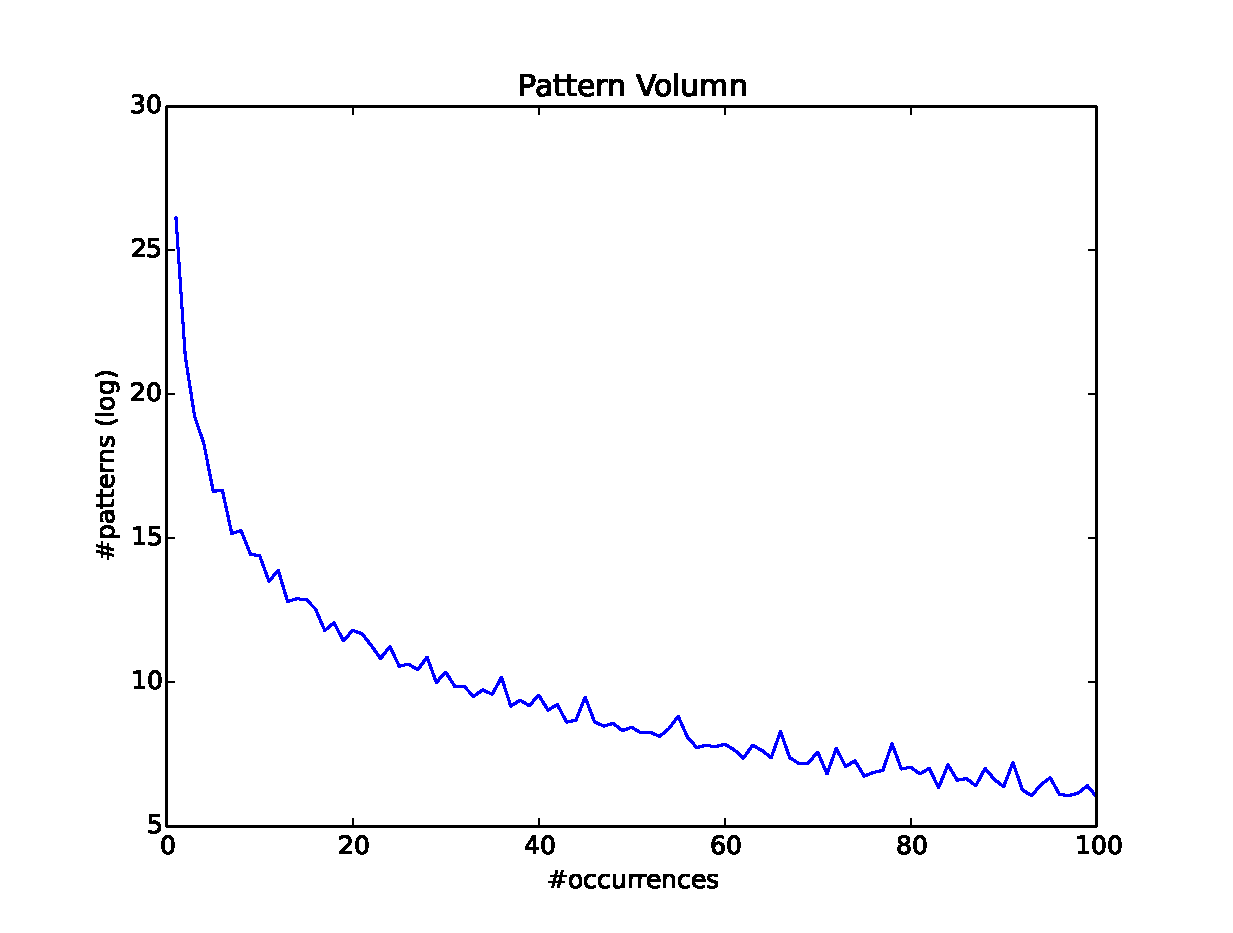
\includegraphics[width=3.2in,height=1.8in]{pv.eps}
\label{fig:pv}
\caption{The Distribution of Pattern Volumn}
\end{figure}
In essense, each relation is characterized by a set of features (patterns or say expressions) collected through DS. 
To express the semantics of a relation between two entities, human beings can think up infinite expressions 
but the number of mentions in our training set is finite and thus it is impossible for collected expressions to cover all the possible expressions. 
With those strict, binary features which have no good generalization properties, our model is determined to miss a lot of novel relation instances. 
As an example, in my held-out evaluation, the number of held-out instances of relation 'Location.contains' that appear in testing corpus is about $31,643$. 
After filtering out instances whose features have no intersection with features of training data, the number of remaining instances decreases to about $17,192$. 
This observation tells us the reason of low recall. 



\section{Related Work}
Mike et al~\cite{mintz} proposed the paradigm of DS for relation extraction which opened one door for this research topic even though the method itself is quite simple and has many problems to be addressed. 



Many works mainly focus on improving the quality of training data generated by DS. 
One genre is using a generative model to re-estimate the association between patterns and relations in a unsupervised manner expecting that some false positive examples will be removed from a relation's pattern collection and some false negative will be explained by some considered relation  
due to the similarity between patterns (the intrinsic structure)~\cite{takagenerative, yaolda, topicmodel}. 
Another genre integrates this intuition into original discriminative model by multi-instance learning~\cite{riedel, hoffmann, surdeanu, 4layers}. 



Those generative models seem complex but the underling intuition is very straight. 
For instance, in Takamatsu et al~\cite{takagenerative}'s model, both relations and patterns are characterized by their associated entity pairs. 
Specifically, let's denote the entity pairs of relation $r$ as $E_r$, the entity pairs of a pattern $s$ as $E_s$. 
Intuitively speaking, if we rank a relation $r$'s associated patterns by $\frac{\vert E_s \cap E_r \vert}{\vert E_s \vert}$ in descending order, the top-ranked ones are more likely to express $r$. 
The more similar a pattern's entity pairs are w.r.t top-ranked patterns' entity pairs, the more likely for it to express $r$ and vice versa. 
Representing a pattern in such a manner allows us to compare different patterns. 
Another benefit is that although entity pairs are ambiguous in many cases, a pattern expresses only one meaning. 
Yao et al~\cite{yaolda} treats a document as a distribution over relations. 
When a relation $r$ is generated, it is responsible for explaining the features, source entity's type, destination entity's type. 
Then the entity type specific distribution is used to sample observed entities. 
This generative story makes a lot of sense but in my opinion, the most important contribution is breaking down original patterns into fine-grained features which are explained by a relation respectively. 
Patterns which are regared as independent objects in original DS now can be compared, 
or say that patterns are represented as fine-grained features and thus co-occurrences of these features contribute to similarity between patterns. 



As for multi-instance learning genre, they are based on the relaxed assumption that if $\exists r(e_1, e_2)\in\Delta$, \emph{at least one} of $(e_1, e_2)$'s mentions express $r$. 
In most cases, this kind of models for relation extraction have a hidden layer of random variables to model the mention level labels 
and a layer of random variables to model entity level labels which are influenced by mention level labels in a aggregation manner. 
The entity level is used to inject supervision into the model. 
To reflect the 'at-least-one' assumption, Riedel et al~\cite{riedel} proposed to model the event that whether the $i$-th mention of an entity pair expresses a relation $r$ by a binary hidden variable $Z_i$. 
Hoffmann et al~\cite{hoffmann} proposed the \emph{MultiR} which is used as baseline in many related works. 
In their model, each mention is associated with a random variable taking value from $R\cup\{\text{OTHER}\}$. 
Then entity level labels are modeled in a binary vector random variable $\mathbf{Y}$ where $Y^{r}=1$ means this entity pair has relation $r$ and vice versa. 
The relationship between hidden layer variables (mention level) and entity level variable is simply a deterministic-or instead of any complex conditional probability distribution. 
The deterministic-or relation is beneficial for simplifing inference procedure but is not able to describe the scenario where appearrance of $r$ at mention level frequently co-occurs with appearrance of $r'$ at entity level. 
Surdeanu et al~\cite{surdeanu} proposed a three layer model which seems similar with MultiR but given an observation (a feature representation of a mention), it predict which relation this mention expresses by a logistic regression classifier and then use $\vert R\vert$ logistic regression classifier to predict entity level labels according to all the mention level labels respectively. 
In such case, a mention level prediction in which only 'Born-in' is activated may also have opportunity to trigger 'Live-in' label at entity level if for most entity pairs, there exists a strong correlation between them. 
Min et al~\cite{4layers} advance further to seperate entity level labels into two layers, one as hidden layer modeling the predictions, one as observed supervision. 
By allowing an inconsistent states between the hidden layer of entity level and supervision, an entity pairs may be associated with some relation which is supported by mention level labels rather than existed ground truth provided by KB which seems helpful for alleviating the influences made by incompleteness of KB. 
Takamatsu et al.~\cite{takamatsu} pointed out that $91.7\%$ entity pairs appear only once in Wik articles. 
In such case, the 'at-least-one' assumption is equivalent to original DS assumption for these multi-instance learning approaches. 



Another interesting work intending to reduce false nagative examples leverages passage retrieval~\cite{passageretrieval}. 
Firstly, sentences w.r.t. a relation $r$ are divided into three categories: 
\begin{itemize}
\item $POS(r)=\{s\in\Sigma\vert{}s\text{ contains some }(e_1,e_2)\text{ where }r(e_1,e_2)\in\Delta\}$ 
\item $RAW(r)=\{s\in\Sigma\vert{}s\text{ contains some }(e_1,e_2)\text{ satisfing }r(E_1, E_2)\}$ 
\item $NEG(r)=\{s\in\Sigma\vert{}s\text{ contains some }(e_1,e_2)\text{ satisfying }r(E_1, E_2)\text{ and }\exists{}e'\text{ s.t. }r(e_1,e')\in\Delta\text{ and }r(e_1,e_2)\notin\Delta\}$ 
\end{itemize}
Then a passage retrieval component (given a relation $r$ as query, retrieve sentences that are most likely to express $r$) is trained with positive examples $POS(r)$ and negative examples $NEG(r)$. 
They use this component to select ``relevant'' passages (i.e., sentences) from $RAW(r)$ and then select entity pairs from these top-ranked sentences. 
Selected entity pairs are added into KB to alleviate its incompleteness. 
When a relation $r$ is a $1$-to-$n$ relation and our KB misses $r(e_1, e_2)$, the principle for constructing $NEG(r)$ is still likely to include false negative examples. 



According to previous analysis, a fine-grained NER tagger is helpful for disambiguating several possible relations of a mention. 
Xiao et al~\cite{112nertag} proposed an approach to tag words with subsets of the universal entity type set which consists of 112 NER tags (multi label). 
Specifically, the 112 NER tags are Freebase types that contain at least $5$ instances (entities). 
Their training set is built by DS where the anchors of Wiki articles are the source of information. 
In detail, a segment of words with an anchor (hyperlink directs to the corresponding Wiki article of an entity) is labeled by Freebase types associated with the entity to which the anchor refers. 
Zhang et al~\cite{xingxing} is the first one to apply the fine-grained entity types for relation extraction task. 
However, their features are traditional mention features and context features but the relation information has not been made full use. 



Up to now, all these approaches discussed made use of strict binary features which can't be generalized well. 
To tackle the sparseness of feature space, word embedding related techniques are imported to relation extraction during the last two years. 
Chen et al~\cite{cdq} propose to represent an entity by the average of its words' vector representation, a relation by the parameters of a neural tensor network. 
Given an entity pair $(e_1, e_2)$, a score of how plausible they are in a certain relationship $r$ is computed by 
$g(e_1, r, e_2)=U^{\mathrm{T}}tanh\{e_{1}^{\mathrm{T}}W_{r}^{1:k}e_2+V_{r}\begin{bmatrix}e_1\\e_2\\\end{bmatrix}+b_{r}\}$ where 
$e_{1}^{\mathrm{T}}W_{r}^{1:k}e_{2}$ results a $k$-dimensional vector $h$ where 
$h_{i}=e_{1}^{\mathrm{T}}W_{r}^{i}e_2$. 
To estimate the parameters describing a certain relation $r$, they acquire supervision directly from adopted KB. 
The intuition is quite simple, any ground triple in KB should achieve a larger score than any invalid triple which 
is constructed by fixing $e1, r$ and randomly selecting a corrupted entity $e_c$. 
Weston et al~\cite{embedding} also leveraging word embedding related technique especially a reasonable geometrical explaination of how a relation connects two entities
which seems difficult to express in a traditional model. 
In their model, constraints for parameter estimation are drawn from both DS and KB. 
Firstly, a mention-relation pair is scored by $S_{m2r}(m, r)=\mathbf{f}(m)^{\mathrm{T}}\mathbf{r}$ where 
$\mathbf{f}(m)=W^{\mathrm{T}}\boldsymbol{\Phi}(m)$ and $\mathbf{r}$ is the embedding of relation $r$. 
The matrix $W$ consists of all the distributed representations of words and $\boldsymbol{\Phi}(m)$ is 
the binary representation of $m$ (a mention is a size-$k$ window here). 
To estimate the parameters, DS heuristically labels mention-relation pairs. 
Then the constraints are $\forall i, \forall r'\neq r_i, \mathbf{f}(m_i)^{\mathrm{T}}\mathbf{r}_i > 1+\mathbf{f}(m_i)^{\mathrm{T}}\mathbf{r}'$
The most important point proposed in their work is to regard a realtion $r$ as a \emph{translation} from source entity's vector $\mathbf{h}$ to destination entity's vector $\mathbf{t}$ .
This intuitive geometric explaination naturally inspired them to minimize 
$S_{kb}(\mathbf{h},\mathbf{r},\mathbf{t})=\Vert \mathbf{h}+\mathbf{r}-\mathbf{t} \Vert_{2}^{2}$. 
Specifically, they adopted a ranking loss, say that appling $S_{kb}()$ to any ground truth triple should result a score 
which is larger than one plus a score generated by appling $S_{kb}()$ to a corrupted triple. 



I also surveyed works on knowlege base population (KBP)~\cite{overviewkbp10, kbp12nyu, cunvkbp10}. 
The KBP contest is so relevant with relation extraction. 
It mainly consists of two sub-tasks:
\begin{itemize}
\item Entity Linking: given a name, decide whether this name corresponds to an entity in a database and, if so, which one. 
\item Slot Filling: given an entity and a attribute of it, determine from a large corpus the values of the specific attribute (some attributes are multi-valued). 
\end{itemize}
Heng et al~\cite{overviewkbp10} gave an overview of TAC 2010 KBP track. 
For entity linking, they pointed that 
\begin{itemize}
\item unsupervised learning can achieve comparable performance as supervised learning. 
\item semantic features such as synonys and variants are helpful. 
\item Wikipedia's structure such as anchors, redirects and disambiguatioin should be made full use. 
\end{itemize}
For slot filling, they gave the following points:
\begin{itemize}
\item coreference and cross-slot inference are necessary because $39.6\%$ answers require system to go beyond single sentence extraction and attribute has many different expressions (e.g., 'son' is 'child'). 
\item external knowledge, although extremely huge covers limited slot fillers (consistent with my observation). 
\end{itemize}
For my best knowledge, Chen et al~\cite{cunykbp10} is the first one to emphasize that 
the slot filling results as feedback are helpful for improving the entity linking task. 
Besides, they gave an interesting approach for integrating these two tasks together. 
Each entity node as well as the given query is characterized by its profile which is defined as 
a list of attributes as well as their value (s).
The value (s) of attributes of an entity node are harvested by slot filling. 



Most approaches on relation extraction process tens of relations. 
Hoffmann et al~\cite{learn5000} proposed a method to collect relation instances for about 5000 relations. 
Although their setting is not identical as normal relation extraction, enriching lexicon as a feature and 
leveraging info-box of Wiki are valuable points for relation extraction. 



%Original DS leads to many false positive examples which may dilute the discriminative capability of useful features. 
%For instance, consider sentences ``Michael Jackson was born in Gary.'' and ``Michael Jackson moved from Gary.'', 
%suppose ``place\_of\_birth(Michael Jackson, Gary)'' is included in adopted KB, 
%since both of the two sentences contain the entity pair (Michael Jackson, Gary), features calculated from the two sentences are combined and labeled with ``place\_of\_birth''. 
%Obviously, the second mention does not express the labeled relation and thus contributes bad pattern to the labeled relation. 
%To alleviate such problem, Riedel et al.~\cite{riedel} relax original assumption to: if an entity pair participate in a relation, 
%\emph{at least one sentence} that mentions the pair might express that relaton. 
%In their model, each entity pair has a random variable $Y$ taking value from $R\cup{}\{\text{NA}\}$ and each mention of the entity pair has a binary random variable $\mathbf{Z}_i$ which is activated 
%if this mention indeed expresses the value of $Y$. 



%Inspired by such multi-instance learning model, \emph{multi-instance multi-label} model is proposed to handle relation overlapping. 
%For example, ``Founded(Jobs, Apple)'' and ``CEO-of(Jobs, Apple)'' are not exclusive. 
%The entity pair (Jobs, Apple) possesses both the two relations at the same time while Riedel et al. constrained each entity pair to only one relation ($Y$ for each entity pair) 
%which is not reasonable. 
%In Hoffmann et al.~\cite{hoffmann}'s model, each entity pair has a $\vert{}R\vert$-dimensional random variable $\mathbf{Y}$ ($\mathbf{Y}^{r}=1$ means the entity pair has relation $r$) instead of a single $Y=r$. 
%The label of this level is aggregated from the labels of mention level (each sentence mentions the entity pair has $\mathbf{Z}_j$ taking values from $R\cup{}\{\text{none}\}$) 
%through a deterministic OR operator. 
%The deterministic OR operator reflects the at least one assumption. 
%Surdeanu et al.~\cite{surdeanu} proposed a similar model. 
%Besides of the at least one feature, they also aggregate the labels for entity pairs from labels of their mentions with features that reflects dependencies between different relations of mentions. 
%Suppose all the mentions for ``(Jobs, Apple)'' in our corpus express the relation ``CEO-of'', 
%since the weak supervision is provided through labels of entity pair $\mathbf{Y}$ and adopted KB activates both $\mathbf{Y}^{\text{CEO-of}}$ and $\mathbf{Y}^{\text{Founded}}$, the former model may 
%make the mention level classifier associate some mention with ``Founded'' while the latter one may correctly classify all mentions 
%and keep $\mathbf{Z}$ and $\mathbf{Y}$ consistent by observing that $\mathbf{Z}_{j}=\text{``Founded''}$ and $\mathbf{Z}_{j}=\text{CEO-of}$ are generated jointly in many cases. 



%Min et al. add one layer to previous 3-layer multi-instance multi-label model. 
%The added layer ($\mathbf{l}$) models the relations of a entity pair. 
%Different from modeling and providing supervision at the same layer, they allow the supervision $\mathbf{y}_{i}^{r}=\text{Unlabeled}$ but $\mathbf{l}_{i}^{r}=\text{Positive}$. 
%Specifically, for an entity pair which does not appear in any relation in KB, its supervision $\mathbf{Y}=\mathbf{0}$ strongly suggests 
%that patterns extracted from mentions of the entity pair indicates ``none''. 
%In this model, the supervision is relaxed. 
%Patterns extracted from mentions of such entity pair also have opportunity to indicate a certain relation. 
%In a word, the 4-layer multi-instance multi-label model tend to make better use of unlabeled cases. 



%As you can see, all the above approaches ignored the false negative produced by both assumption of DS and incompleteness of KB. 
%Xu et al.~\cite{xu} propose a novel labeling strategy which leverages the entity types. 
%They divided sentences with respect to a relation $r$ into three classes: 
%\begin{itemize}
%\item $POS(r)=\{s\in\Sigma\vert{}s\text{ contains some }(e_1,e_2)\text{ where }r(e_1,e_2)\in\Delta\}$ 
%\item $RAW(r)=\{s\in\Sigma\vert{}s\text{ contains some }(e_1,e_2)\text{ of required types of }r\}$
%\item $NEG(r)=\{s\in\Sigma\vert{}s\text{ contains some }(e_1,e_2)\text{ of required types of }r\text{ where }\exists{}e_j\text{ such that }r(e_1,e_j)\in\Delta\text{ and }r(e_1,e_2)\notin\Delta\}$
%\end{itemize}
%Then a passage retrieval component (given a relation $r$ as query, retrieve sentences that are most likely to express $r$) is trained with positive examples $POS(r)$ and negative examples $NEG(r)$. 
%They use this component to select ``relevant'' passages (i.e., sentences) from $RAW(r)$ and then select entity pairs from these top-ranked sentences. 
%Selected entity pairs are added into KB to alleviate its incompleteness. 
%However, the entity pairs in $NEG(r)$ may be caused by incompleteness of KB itself. 
%Besides, $POS(r)$ are labeled according to original DS assumption as well as entity type requirement which is not always reliable as the ``(Micheal Jackson, Gary)'' example showed. 



%Takamatsu et al.~\cite{takamatsu} pointed that $91.7\%$ entity pairs appear only once in Wikipedia articles. 
%In such case, the at least one assumption is equivalent to original DS assumption for those multi-instance learning approaches. 
%Takamatsu et al. proposed a generative model to predict whether a pattern (they define a pattern as entity types as well as the sequence of words on the path of the dependency parse tree between the two entities such as ``[Person] born in [Location]'') express a target relation. 
%Intuitively, in our corpus, the entity types in a pattern will be instantiated by both entity pairs that are covered by KB and entity pairs that are unknown. 
%If the number of the former kind of entity pairs is much larger than the latter kind of entity pairs, the pattern is very likely to be associated with corresponding relations. 
%Thus we can revise some wrong label of unknown relation instances. 



%\section{Critical Factors}
%For simplicity, existing approaches made use of Stanford's named entity tagger which has only four broad entity types \{person, location, organization, miscellaneous, none\}. 
%In fact, most relations connect two entities where the entities belong to specific entity types such as ``compose(musician, song)''. 
%Besides, a relation can be expressed by various sentences but the entity types is much more stable which means that 
%entity type is discriminative to distinguish relatinos. 
%Someone may argue that named entity recognition (NER) is not easier than relation extraction and thus we can not treat NER as a subproblem of relation extraction. 
%Indeed, how to associate an entity to appropriate entity type is coupled with relation extraction. 
%Without the context, given that ``Apple'' is an organization and ``Jobs'' is a person, we will guess the entity pair is connected by relation ``CEO-of''. 
%Inversely, given ``product-of(ipad, Apple)'', we will guess that ``Apple'' is a company rather than one kind of fruits. 
%Generally speaking, the relaion between an entity and its type is \emph{isA}. 
%Given that ``isA($e_1, E_1$)'' and ``isA($e_2, E_2$)'', the most popular type of edges (i.e., relations) between hyponyms of $E_1$ and hyponyms of $E_2$ is a good choice for connecting $e_1, e_2$. 
%
%
%Feature space is extremely sparse because the lexical and syntactic features change in different mentions of different relations. 
%This is one of the reasons why Xu et al. use coarse features for training passage retrieval component. 
%Takamatsu et al. define a pattern in that way so that variation of argument entity pairs is eliminated (only reqire matching of the entity type). 
%
%
%Original DS as well as those 3-layer multi-instance learning models suffer from incompleteness of KB. 
%The false negative examples make it difficult to classify one mention to appropriate relation 
%because sharing common features between negative examples and positive examples reduce the importance of these features which actually belong to positive examples. 
%The above 4-layer models seperate week supervision provided by KB from true labels of an entity pair 
%so that unlabeled pairs are allowed to have not existed relations which may be more consistent with their mention level labels. 
%However, there is still no a reasonable way to describe the dependencies between observed supervision and the layer that models labels of entity pairs. 
%Besides, as a multi-label classifier, for a certain relation, we actually regard all the other relations as well as the ``OTHER'' relation as negative examples for it. 
%However, relations are not exclusive. 
%Multi-instance learning methods can not address such problem when the given entity pair appears only once in our corpus. 
%In such cases, which relation will this mention be assigned is
\bibliographystyle{abbrv}
\bibliography{survey}
\end{document}

